\chapter{Design}



\section{Overall Architecture}



\section{Mapping}
The central component of the application was going to be a map. For this reason it was vitally important that an appropriate mapping solution was used.

\subsection{Google}
Google provides a simple, easy to use interface to their own maps making it the obvious choice for any Android application. Their maps are accurate, up-to-date and very detailed.

Google Maps were used for early prototype development.

Unfortunately there are a number of restrictions in place stopping their use in a number of situations. The most relevant of which is that they can not be used in an application that is not freely available to the public. Therefore restricting it's use in a paid-for application, such as MapWars may become. As the future of the application is uncertain it seemed desirable to steer clear of as many possible restrictions as possible. For this reason it was important to find a comparable alternative.

\subsection{OpenStreet Map}
OpenStreet map is an INSERT DESCRIPTION OF OSM HERE. It's growing popularity means that INSERT STATS ABOUT AREAS COVERED. With an acceptable level of detail combined with it's open SOMETHING(ethos?) made it the next most obvious source.

OSM has an API that allows it to be easily embedded into webpages but no native android SDK. A number of 3rd party libraries are available. The most complete and popular is that provided by MapQuest.

MapQuest are a mapping company that combines proprietary data and OSM data to create their own maps. They offer an Android SDK that gives you the option of which tile source to use. There are obviously restrictions to the proprietary data but if you opt for the free tiles then the same license is used as with OSM. The Android SDK available was designed to mirror the API available for the Google Map SDK. This made swapping out the Google Maps code and replacing it with the MapQuest code was trivial and problem free.

At the point in time of implementing MapQuest the design had called for the option to switch between satellite and road maps. MapQuest's main drawback, and more widely OSM itself, was it's lack of detail. The level of zoom supported was a number of levels less than that of Google Maps. These extra zoom levels would have made unit manipulation easier on smaller devices. Satellite images were the main concern as they were not available at the level of zoom required to make game play comfortable.

MapQuest was used as the mapping solution for a large portion of development and offered a stable platform. Once more of the functionality was in place user testing presented a number of problems with the map tiles being used. Most significant of which was a difficulty in being able to locate units among the details presented with the map. The sprites and colours being used to represent units were experimented with but none were clearly visible. The problem was with the design of the tiles being used and not necessarily the zoom levels present, although this may have helped alleviate the problems.

\subsection{MapBox}
One option available was to use a tile creator and host the map tiles on a server. This would be a costly and difficult solution to the problem. Hosting tiles is not a trivial task and require large amounts of storage and bandwidth.

MapBox offer beautiful hosted tiles. They also have their own software called TileMill which allows the creation of bespoke tiles based on any data source which can then be hosted and distributed via their network. TileMill was based on a CSS style syntax allowing you to customise any visual aspect, from line widths, colours, strokes. It also had the ability to import data from any source giving the ability to build up rich tiles with as much detail as required. For MapWars only the most basic detail was required while using a simple colour pallet. The idea was to make any unit stand out against the map while still presenting all the information required to orientate the user with their surroundings. 

Tiles could be loaded from MapBox using a standard URI syntax used by the most tile vendors. This allowed it to integrate easily into any mapping framework.All that was needed was an SDK that allowed custom tile sources. Such functionality was found in OSMDroid. Like with MapQuest, OSMDroid followed the same pattern as Google Maps allowing it to be easily placed into the application without only one substantial problem. OSMDroid was missing one function that was supported by both Google Maps and MapQuest. These function was key in selecting units so had to be reimplemented ... which was not difficult but took time. Assumption was made it would be as effortless as the previous transition. After integration was complete plugging in the URI to my generated tiles was simple and worked straight of the bat.

MapBox did not offer satellite imagery but the beauty and simplicity of the maps being used made up for this. It was also decided that the complexity of such maps would just present the same images as found with the default OSM tiles. Satellite images could always be added to OSMDroid by simply finding a tile source and using that and would have no affect on the functionality of the application. 

\section{User Interface}
When developing any application for a small form factor it is important to consider how the user interface can be minimized, and to not clutter the display making precise controls difficult. This is especially important when trying to fit all the functionality of a \gls{rts} game within the small form factor of a mobile device. To get around this problem only the essential controls will be included with only a portion of these being accessible from the main game screen.

\begin{figure}[H]
\centering
\begin{minipage}{.5\textwidth}
  \centering
  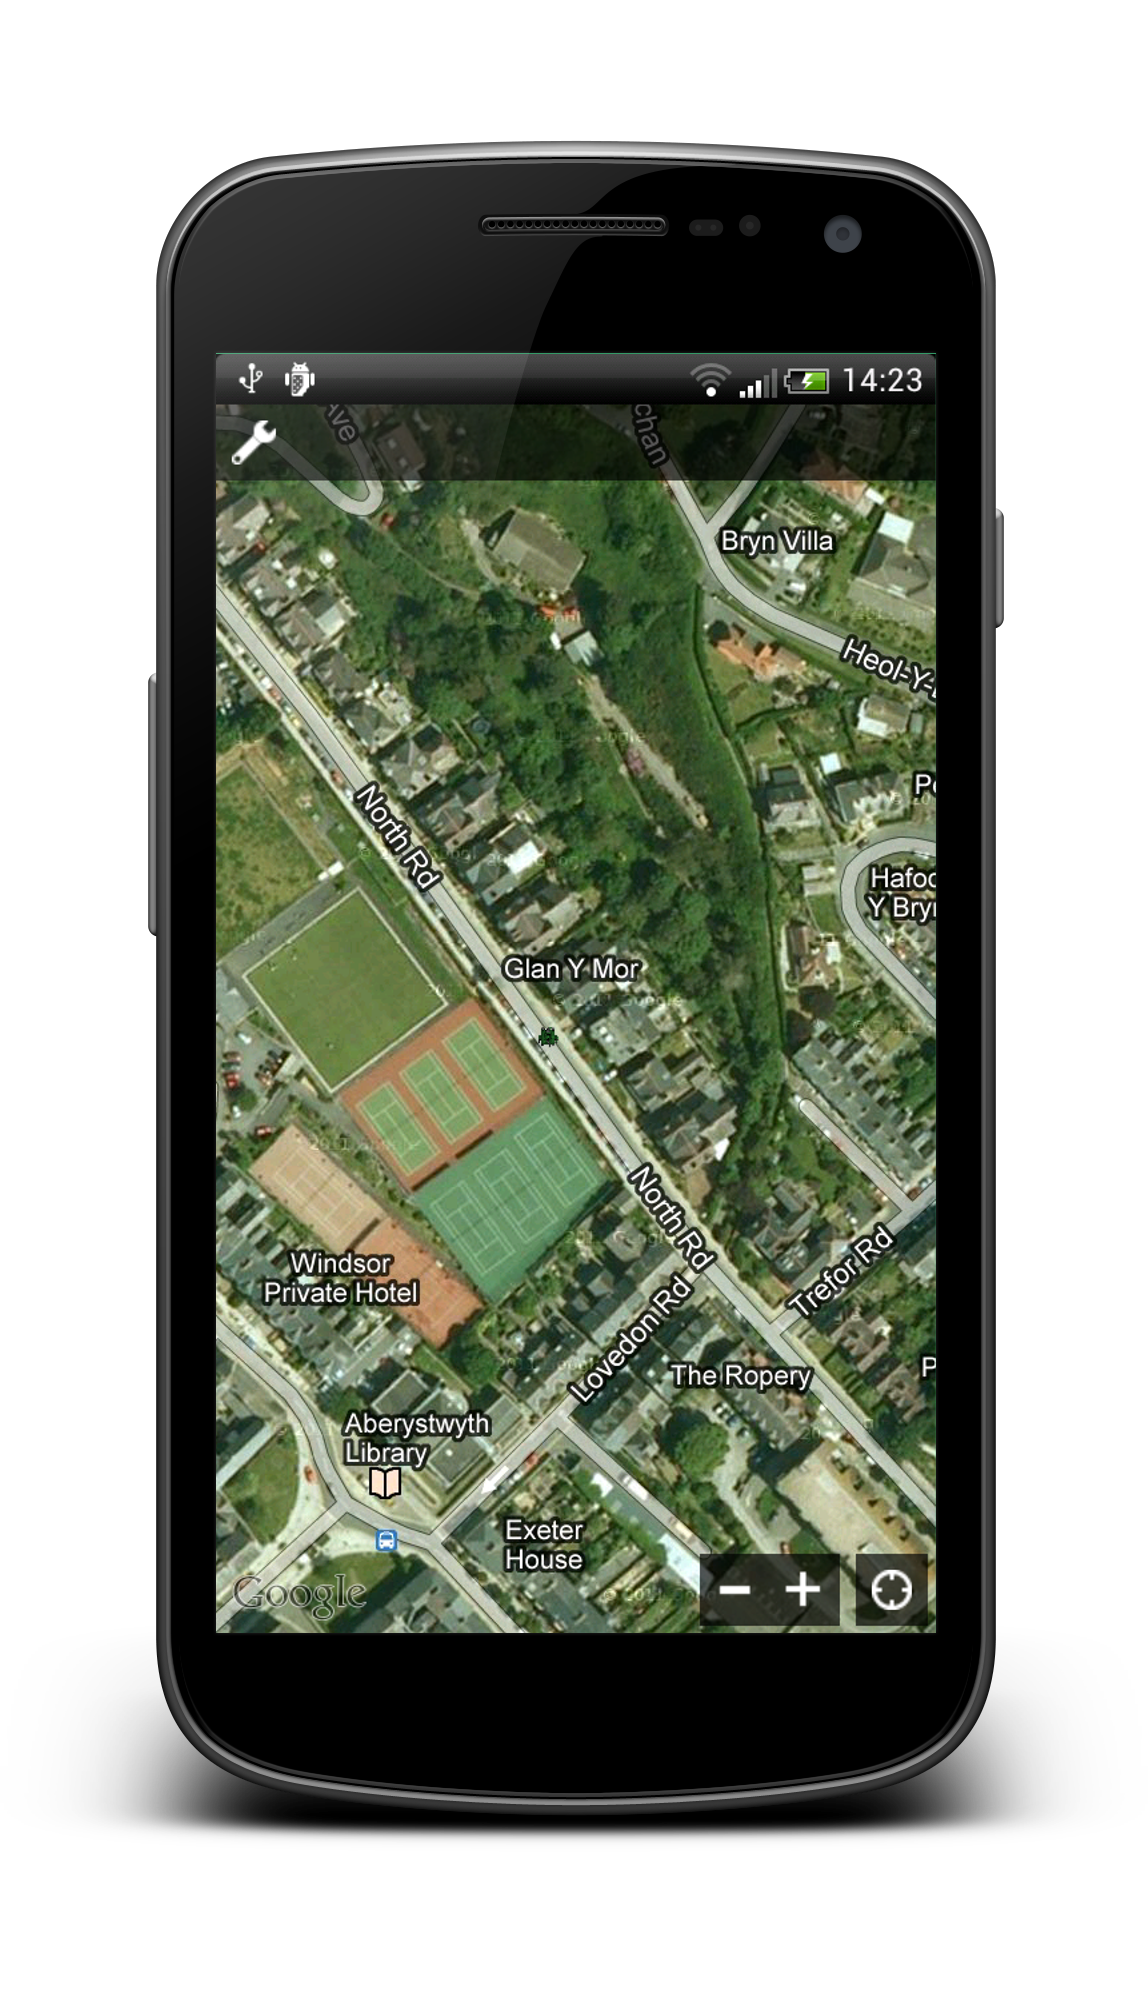
\includegraphics[width=.4\linewidth]{Images/maps-google.png}
  \captionof{figure}{Insert design of game map}
  \label{fig:test1}
\end{minipage}%
\begin{minipage}{.5\textwidth}
  \centering
  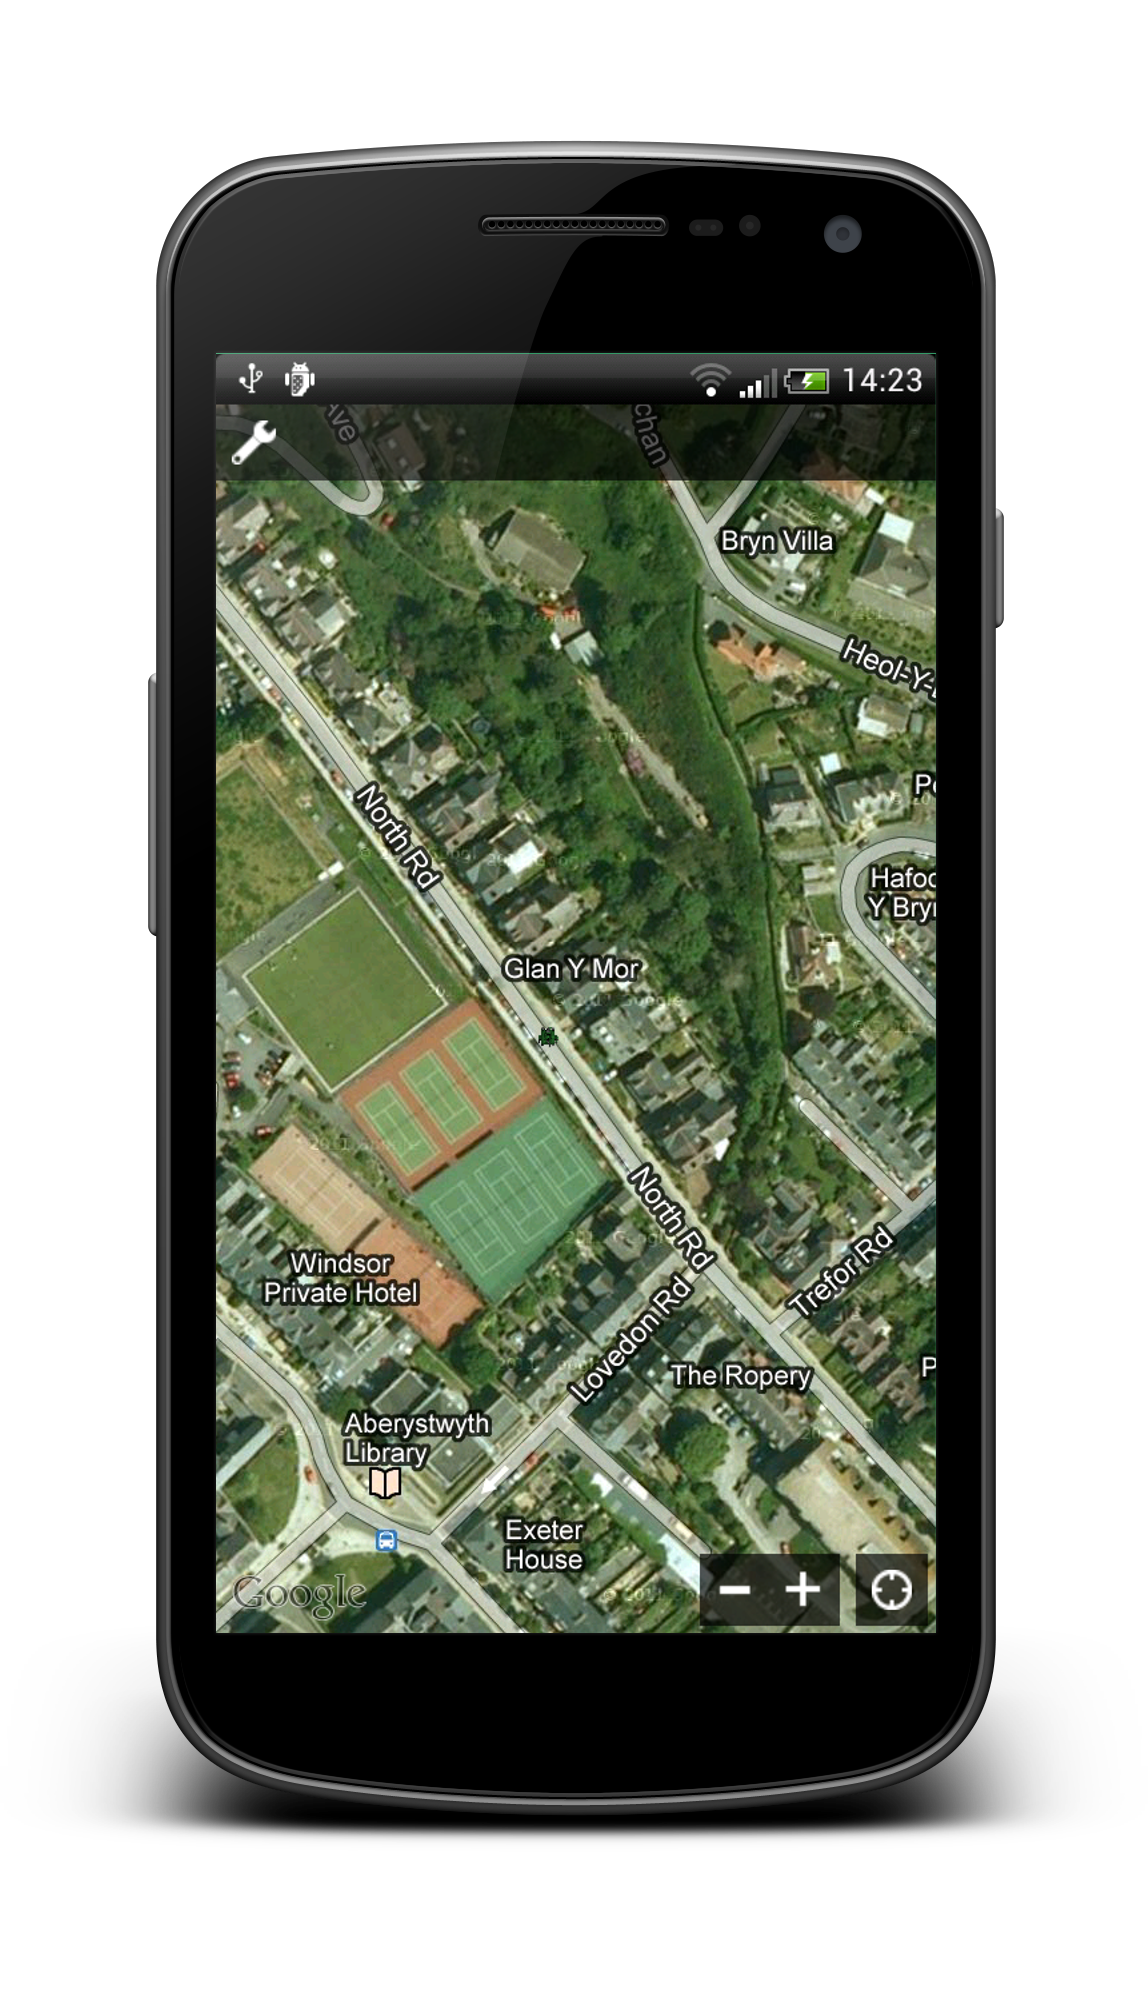
\includegraphics[width=.4\linewidth]{Images/maps-google.png}
  \captionof{figure}{Insert design of game map menu}
  \label{fig:test2}
\end{minipage}
\end{figure}

 Figure \ref{fig:test2}